% This is a default-selection of plugins that are used widely in this repo.

\documentclass[a4paper,10pt,fleqn]{article}
\usepackage[utf8]{inputenc}

% deutsche Trennmuster etc.
\usepackage[ngerman]{babel}
\usepackage[T1]{fontenc}

% mathematical simbols and fonts
\usepackage{mathtools} 
\usepackage{amssymb}
\usepackage{amsmath}
\usepackage{ntheorem}
\usepackage{polynom}
\usepackage{marvosym}
\usepackage{tabu}
\renewcommand*{\bmod}{\mathbin{\%}}
\everymath{\displaystyle}

\usepackage{multicol}
\usepackage{color}
\usepackage[usenames,dvipsnames]{xcolor}
\setlength{\columnsep}{1cm}
\setlength{\columnseprule}{0.25pt}
\def\columnseprulecolor{\color{gray}}
\usepackage{hyperref}

\usepackage[margin=1.5cm]{geometry}
\usepackage{graphicx}
\usepackage{pgfplots}
\pgfplotsset{compat=1.10}

%Code higlighting

\usepackage{minted}

% make lists more compact:
\newlength{\wideitemsep}
\setlength{\wideitemsep}{.5\itemsep}
\addtolength{\wideitemsep}{-5pt}
\let\olditem\item
\renewcommand{\item}{\setlength{\itemsep}{\wideitemsep}\olditem}
\renewcommand{\arraystretch}{1.25}

\title{Zusammenfassung CN2}
\author{Fabian Hauser}
 
\begin{document}
\maketitle

\section{Varia}
10 Seiten A4 Zusammenfassung

\section{Telefonie}

\begin{description}
\item[Data Plane] \hfill \\
	Forward IP-Packets. Z.B. STP, VLANs
\item[Control Plane] \hfill \\
	Routing Protocols, Overlay technologies (MPLS), z.B: Forwarding of Ethernet Frames
\end{description}


\subsection{G.711 / PCM}
 256 Audio-Steps using 8 Bits, Sample 8000/sec (nyquist frequency) = DS0, 64Kbps


\subsection{ISDN}
Braucht NT Wandler.

\begin{description}
\item[S-Bus] \hfill \\
	 Digitaler Bus im Haus; Data Plane.
\item[D-Kanal] \hfill \\
	Synchronisierungs-Kanal zur Dorfzentrale
\item[PBX] \hfill \\
	Die Dorfzentrale; Übersetzt Rufnummer-Anfragen (Wählton) zu weiteren Zentralen

\end{description}

\subsection{SS7}

Ähnlich BGP ist das SS7 Routing Protokoll die Verbindung zwischen allen Telefonzentralen.
	
\subsection{Voip}
Läuft über Router; muss von Telefonnummer eine IP-Addresse "extrahieren".
	
\subsubsection{The Connection / Bearer Plane}
Switching Logic: Connection Negotiation, Transcoding

Mittels z.B. SIP mit CCP Verbunden.

\subsubsection{The Call Control Plane: SIP as a Example}
Call Logic: Signalling \& Call control
Logic / Services

Mittels z.B. TAPI / INAPI mit Services Plane verbunden.

Distributed call processing: (SIP, H.323), Centralized cal process (SCCP, MGCP, MEHACO, H.248)

Inititation von Verbindungen

\subsubsection{The Services Plane}
Service Logic: IN Service Logic, AAA, Address Resolution


\subsection{Session Description Protocol SDP}
Manage the Lines respectivly connection properties

\begin{description}
\item INVITE \hfill \\
	codecs support etc.
\item REGISTER
\item BYE
\item ACK 
\item CANCEL
\item OPTIONS
\end{description}

Mediaübertragung über RTP.

\subsection{SIP}

\begin{itemize}
	\item User location
	\item User availability
	\item User capabilies
	\item Session setup
	\item Session management
\end{itemize}

Makes use of:
\begin{itemize}
	\item HTTP
	\item SDP
	\item RTP / RTSP
	\item URI / URL
	\item DHCP / DNS
	\item MIME
	\item TLS / IPSec
\end{itemize}

\begin{description}
	\item Registrar Server \hfill \\
		Datase of IP / Numbers matching of the User Agent
	\item Proxy \hfill \\
		Routing of SIP signalling messages
	\item Redirect Server \hfill \\
		Redirects von Anrufen
\end{description}

\section{Routing}

Layer 3, dynamisch oder statisch

\subsection{Routing Hierarchy}

Separiert in \emph{Autonomous Systems} (AS). Zwischen den AS wird mit \emph{Exterior Routing Protocols} (EGP) benutzt, üblicherweise BGP.

Innerhalb der AS wird ein Interior routing Protocol (IGP) verwendet.

\subsection{Distance Vector}

Es wird jeweils die ganze Tabelle zurückgegeben.

\subsubsection{Split Horizon}

Der Router, welcher die Route mitgeteilt hat, wird nicht "wiederholt".

\subsection{Link State Protocol}

\begin{enumerate}
	\item Ermittlung Nachbarn mit Hello Protocol
	\item Kenntnisse Nachbarn weitergeben. (\emph{Link State Advertisments})
	\item \emph{Shortest Path First} nach kenntniss von ganzer Datenbank
\end{enumerate}

Es wir jeweils nur ein Single Entry durchgegeben, mit dem Inhalt (RouterID, NeighborID, Cost)

\subsubsection{Shortest Path Algorithm}

\begin{enumerate}
\item %TODO	
\end{enumerate}


\subsection{OSPF}

\begin{itemize}
	\item Secure (Signing)
	\item Classless
	\item Max 50 client per Area
\end{itemize}


\subsection{BGP}

Border Gateway Protocoll

\subsubsection{Autonomouse Systems}

1-65535 unique
private AS pool from 64512 to 65535 (similar to private IPs)
RFC 6793 introduces 32 bit AS numbers
(y.x), each x/y = 16bits
BGP4, is used to interconnect AS

\subsubsection{Connection}

\paragraph{Home} \hfill \\

Access to ISP; default route

\paragraph{Multi-Homed} \hfill \\
Connected with muliple AS Provider or multiple Links to the same Provider

\begin{description}
	\item[Transit AS] \hfill \\
	Can be used for transit traffic by other providers
	\item[Nontransit AS] \hfill \\
	Advertises only its own routes to both providers
\end{description}

\subsubsection{Protocol}

The less hops the better

Communicates in which AS are which IP Ranges.

BGP4 supports CIDR and route aggregation

BGP is a Path vector protocol

TCP Port 179

\begin{enumerate}
	\item OPEN MESSAGE: Exchange AS, router ID, holdtime, Capability negotiation
	\item NOTIFICATION (Example: ''peer in wrong AS'')
	\item KEEPALIVE when no updates
	\item UPDATE (incremental)
\end{enumerate}


Netze werden explizit Withdrwan

Attributes: Pfadlängen, Kosten etc.

Prefixes: Neuer Weg etc.

\subsubsection{Types}
(\emph{Nicht} zum auswendig-lernen)
\begin{description}
	\item[1: ORIGIN]
	\item[2: AS-PATH]
	\item[3: NEXT-HOP]
	\item[4: MED] Multi Exit Discriminator (Reccomandations Traffic ports)
	\item[5: LOCAL\_PREF] Local preferences
\end{description}

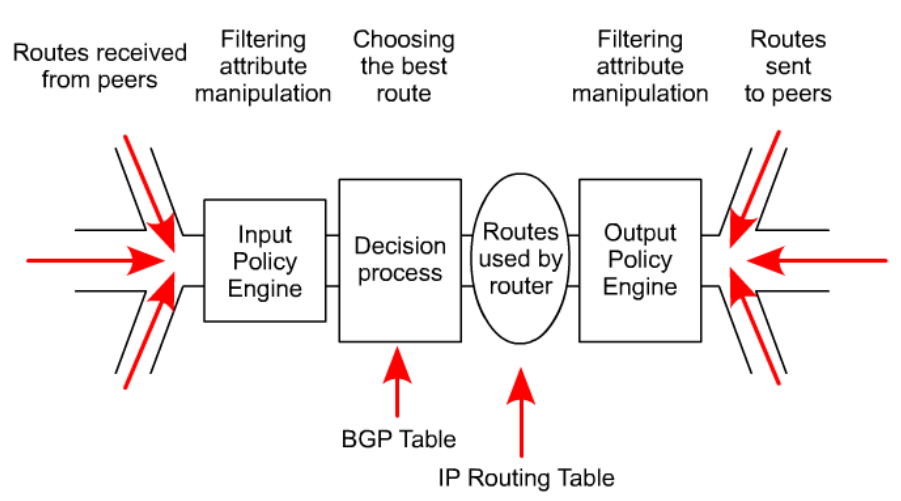
\includegraphics[width=0.5\linewidth]{img/bgp_process_model.png}

\subsubsection{Peering vs. Transit}

Transit: Kostet, quasi default gateway wo via peering nicht abgedeckt.
Peering: Lokale Provider verknüpfen. (üblicherweise Gratis).

\paragraph{Peering}
Multi-lateral Peering: Zentrale Einheit welche das Peering organisiert (Zentraler Swtich)

Bi-lateral Peering: Direktes Peering mit anderem Provider.


\section{IP}

\subsection{Multicast}

Single Sender, Multiple Receivers. Darum UDP mit entsprechenden Nachteilen.


Multicast Adressen sind zwischen 224.0.0.0 bis 239.255.255.255 bei IPv4.

Link Local Adrdres: 224.0.0.0 - 224.0.0.255
Global Address Range: 224.0.1.0-238.255.255.255
Administratively Scoped Address Range (Privately used addresses within private multicast domain): 239.0.0.0 - 239.255.255.255



\subsubsection{MAC Layer 2}
	Es gibt auch Multicast-Mac-Adressen 00-00-00 bis 01-00-5e-7f-ff-ff.
	Es werden jeweils die letzten 23-Bit der IP an 01-00-5e- angegängt.
	
	Von der IPv4 Adresse werden die ersten neun Bits abgehackt.

\subsubsection{IGMP}

Internet Group Management Protocol

Local LAN to Router, wished group memberships.

IGMPv3: Join / Leave to/from explicit sources and broadcast addresses.

\subsubsection{Wide Area}
üblicherweise PIM

\subsubsection{Multicast Distribution Trees}

Zur verhinderung von Loops.

Shortest Path oder Source Tree bei einfachen Trees
-> More memory n(S x G) but optimal paths,


Shared Tree (PIM-Sparse Mode): PIM Rendezvous Point 
-> Less memory n(G) but no optimal paths. The client can afterwards directly connect tothe source

\emph{(source,dest)}
Z.B: \emph{(*, 224.20.10.1)}

\subsubsection{RPF}

Reverse Path Forwarding

Es wird von der Destionation zur Source einen Weg aufgebaut.

Jeweils zum nächsten Weg zur Source (im Zweifelsfall der ''letzte'' hop richting root.

Dense Mode: ''Push'' model: traffic floded through net. Can be unsubscribed with ''Prune''

Sprase-mode: ''Pull'' model: traffic on subscription. Client connects to Randevouz Point, The Source also Informed the RP.

\subsubsection{IGMPv1-v2 Snooping}

Nur Geräte, welche sich per IGMP subscriben, kriegen vom Switch die entsprechenden Daten.



\section{Wide Area Networks WAN}

Vernetzung von Standorten.

\subsection{Leased line}

Private line between endpoints.

N x 64kbps

Provider does usually Multiplexing.

\paragraph{E1 Framing I.}

32 Slots * 8bits

Möglich, mehre Kanäle per Multiplexing zusammenzuhängen.

\subsection{SDM / TDH}?

\subsection{Synchronous Digital Hierarchy (SDH)}

''Container'' gehen immer im Ring herum. Es gibt eine Spur in jeweils jede Richtung.

Ein Add/Drop Multiplexer Fügt/Entfernt Pakete aus dem Container.

\subsection{PPP}

Layer 2

Point to Point Protocoll

(Sehr ähnlich Ethernet)

Regelt IP Vergabe, Link Configuration, Quality, Error Detection

Authentication, Callback, compression, Multilink

\subsection{Frame Relay}

\begin{itemize}
	\item Layer 2
	\item Macht ein Backbone taugliches ''Ethernet'' im WAN.
	\item Mehrere logische Verbindungen über eine physische Leitung. Dadurch: Bandbreite geshared.
	\item Packet Orientiert
	\item PVC (Permanent Virtual Circuits)
	\item SVC (Switched Virtual Circuits)
	\item Virtuelle Verbindungen werden als: DLCI (Data Link Connection Identifier) bezeichnet.
	\item Es hat 1000 mögliche Adressen
	\item Kennt keine Redundanz etc.
	\item QoS \begin{itemize}
		\item Treffic shaper beim Endpunkt (Steuerung vom Kunden).
		\item Traffic Policer (Harte forcierung vom Provider)
		\item Congestion Flags from Network (FECN, BECN, DE-bit)
	\end{itemize}
	\[
		CIR = \frac{Bc}{Ts}
	\]
\end{itemize}

Addressen haben eine Lokale Signifikatent (Die Nummer beschreibt pro Ziffer den zu wählenden Weg.

\subsubsection{Begriffe}
	%TODO: insert img/frame_relay_...


\subsection{ATM}

\begin{itemize}
	\item Cell based switching.
	\item Wird u.a. von ADSL und UMTS verwendet.
	\item Realtiv schnell (Immer Ethernet etwas voraus im Speed).
	\item Ermöglicht leichtes integrieren von QoS
	\item Schnelles switching da in Hardware realisiert
	\item Erlaubt CBR (Constant Bit Rate)0
\end{itemize}

\subsection{MPLS: Multiprotocol Label Switching}

Vorteile: Skalierung, Plug'n'play, just like an IP net


Features: QoS, Traffic Engineering, OAM/MIBs

Usually: Service Provider, Datacenter Provider

\subsubsection{Working}

Label based routing (the router only knows, where to forward a specific label / interface to.

\begin{description}
	\item[P (Provider) router = label switching router = core router (LSR)] \hfill \\
		Switches MPLS-labeled packets
		Runs an IGP and LDP
	\item[PE (Provider Edge) router = edge router (LSR)] \hfill \\
		Imposes and removes MPLS labels
		Runs an IGP, LDP and MP-BGP
	\item[CE (Customer Edge) router] \hfill \\
		Connects customer network to MPLS network
	\item[Route-Target] \hfill \\
		64 bits identifying routers that should receive the route
	\item[Route Distinguisher] \hfill \\
		Attribute of each route used to uniquely identify prefixes among VPNs (64 bits)
		VRF based (not VPN based)
	\item[VPN-IPv4 addresses] \hfill \\
		Address including the 64 bits Route Distinguisher and the 32 bits IP address
	\item[VRF] \hfill \\
		Virtual routers: Routing of \emph{(TAG)IP}
	\item[FEC] \hfill \\
		is a group of IP packets which are forwarded in the same manner
	\item[LSR] \hfill \\
		Label Switch Router
	\item[LIB] \hfill \\
		Label Information Base (DB of labels)
	\item[GRE] \hfill \\
		IP in IP Verschachteln (unverschlüsselt).
\end{description}

Layering with multiple Labels are possible.


\subsubsection{LDP}

Label Distribution Protocol.

Ähnliches Protokoll: RSVP (reserviert Ressourcen)

\subsubsection{L2TPv3}

Only IP Core is neccessary; no MPLS to allow e.g. Ethernet Virtual Wire Service.

\subsubsection{AToM: Any Technology over MPLS}

Buils on MPLS Core; Wire Connection

Hat VC-Label (VLAN).; Macht Layer 2 über längere Distanzen.

\subsubsection{VPLS}

Virtual Private LAN Service:

MPLS-Core.

Letzte zwei sind heute MPLS Layer-2 VPNs.

Verhinderung von Loop: Spanning Tree wird durch Split-Horizon ersetzt.


\subsubsection{QoS \& Traffic engineering}

QoS-Label from IP is mapped to a MPLS-Label-field.



\end{document}